\section{Learning-based Speculator}
\label{sec:speculation}

\if 0
\begin{figure}
    \centering
    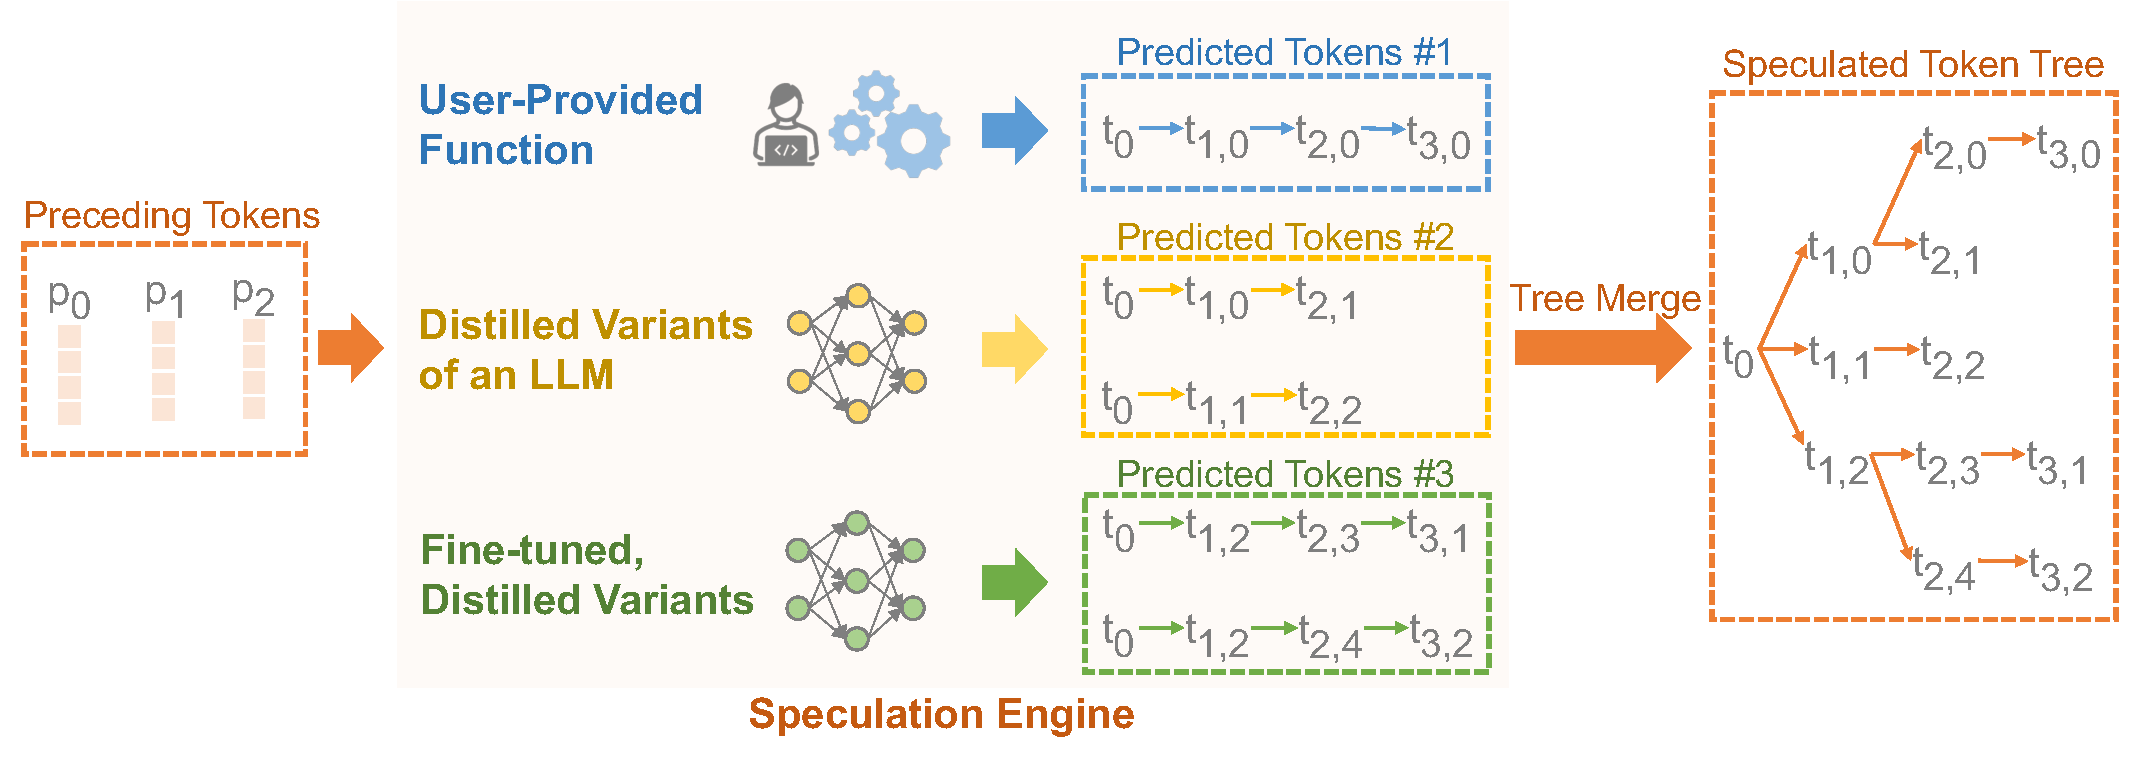
\includegraphics[scale=0.38]{figs/speculation_engine_v2.pdf}
    \caption{An overview of \Sys's speculation engine. \ZJ{To be removed}}
    \label{fig:speculation_engine}
\end{figure}
\fi

\begin{table}
\begin{center}
\caption{\rev{The success rate of verifying a token for \llama-7B using the top-$k$ tokens derived from \llama-68M. The five prompt datasets are described in \Cref{subsec:setup}.}}
%\footnotesize
\label{tab:acceptance-rate}
\begin{tabular}{l|l|ccccc}
\toprule
& Dataset     & $k=1$ & $k=2$ & $k=3$ & $k=4$ & $k=5$ \\ \midrule
\multirow{5}{*}{\rotatebox[origin=c]{90}{\parbox{2cm}{\bf \centering Greedy\\ decoding}}}
& Alpaca     &68\%          & 77\%    & 81\%     & 84\%     & 85\%     \\
& CP         &69\%          & 79\%    & 83\%     & 86\%     & 87\%     \\
& WebQA      &62\%          & 72\%    & 77\%     & 80\%     & 82\%     \\ 
& CIP        &70\%          & 81\%    & 85\%     & 88\%     & 89\%     \\
& PIQA       &63\%          & 75\%    & 79\%     & 83\%     & 85\%     \\
\midrule
\multirow{5}{*}{\rotatebox[origin=c]{90}{\parbox{2cm}{\bf \centering Stochastic\\ decoding}}}
& Alpaca     &54\%          & 81\%    & 91\%     & 95\%     & 97\%     \\
& CP         &56\%          & 82\%    & 92\%     & 95\%     & 97\%     \\
& WebQA      &52\%          & 80\%    & 90\%     & 94\%     & 96\%     \\ 
& CIP        &57\%          & 84\%    & 92\%     & 95\%     & 97\%     \\
& PIQA       &55\%          & 82\%    & 91\%     & 95\%     & 97\%     \\
\bottomrule
\end{tabular}
\end{center}
\end{table}

\if 0
Existing speculative decoding methods perform {\em sequence-based} speculation, where an SSM predicts a sequence of tokens to be verified by an LLM.
%
However, a key limitation of sequence-based speculation is that the alignment between an SSM and an LLM is inherently bounded by the model capacity gap between the two models~\cite{leviathan2022fast, stern2018blockwise}.
%%%
Our preliminary exploration shows that using a larger SSM can achieve better speculative performance at the cost of increased memory overhead and inference latency.
\fi

\rev{Existing speculative decoding methods perform {\em sequence-based} speculation, where an SSM predicts a single sequence of tokens to be verified by an LLM.
%%%
However, a key limitation of a single speculated sequence is that the probability of a successful alignment between the LLM and the speculated token sequence decays exponentially with the expected alignment length.
%%%
This can be further exacerbated by the fact that the speculation only includes a single candidate token to verify per step, resulting in suboptimal speculative performance.
%%%
On the other hand, by encouraging more diverse speculated candidates per step, the probability of a successful match per step (i.e., the token decoded by the LLM is in this candidate pool) can be greatly improved. 
%%%
To this end, \sys aims to construct a tree of speculated candidates by exploiting diversity within a single SSM and across multiple SSMs.
In particular, \sys's {\em learning-based speculator} aggregates the predictions of one or multiple SSMs to maximize speculative performance while maintaining low memory overhead and inference latency.
%
\Sys uses a {\em token tree} to organize the tokens produced by the speculator and introduces two methods for constructing token trees: {\em expansion-} and {\em merge-based} tree constructions.}
%\XM{multiple SSMs or multiple/one SSM?}

\begin{definition}[Token Tree]
A token tree $\m{N}$ is a tree structure, where each node $u \in \m{N}$ is labeled with a token $t_u$, and $p_u$ represents $u$'s parent node in the token tree. 
For each node $u$, $S_u$ represents a sequence of tokens identified by concatenating $S_{p_u}$ and $\{t_u\}$\footnote{For the root node $r$, $S_r$ represents the token sequence $\{t_r\}$.}.
\end{definition}

\rev{\paragraph{Expansion-based token tree construction.}
One approach to creating a token tree involves deriving {\em multiple} tokens from an SSM within a single decoding step.
This approach is motivated by an important observation that when an SSM misaligns with an LLM (i.e., the two models select different top-1 tokens), the token selected by the LLM is generally among the top-$k$ tokens from the SSM for very small values of $k$.
\Cref{tab:acceptance-rate} shows the success rate of verifying a token using the top-$k$ tokens derived from an SSM, where a verification is successful if the token selected by the LLM is among the top-$k$ tokens from the SSM. Compared to only using the top-$1$ token from an SSM, using the top-$5$ tokens can increase the success rate from 70\% to 89\% for greedy decoding and from 57\% to 97\% for stochastic decoding.}

%%%
\rev{Directly selecting the top-$k$ tokens at each step leads to an exponential increase in the number of potential token sequences, which substantially elevates inference latency and memory overhead. Consequently, we adopt a {\em static} strategy that expands the token tree following a preset {\em expansion configuration} represented as a vector of integers $\langle k_1, k_2, ..., k_m\rangle$, where $m$ denotes the maximum number of speculative decoding steps, and $k_i$ indicates the number of tokens to expand for each token in the $i$-th step.
%including the expansion depth and width. Here the expansion depth denotes the maximum number of speculated decoding steps and the expansion width represents the number of selected tokens in each step. 
%In this way, the amount of speculated token sequences is bounded by manageable size. 
For example, \Cref{fig:token_tree_merge} illustrates the expansion configuration $\langle 2, 2, 1 \rangle$, leading to four token sequences.
Our evaluation (see \Cref{subsec:eval_token_tree}) shows that even a simple strategy can generate highly accurate speculative results.
We acknowledge that {\em dynamically} expanding a token tree from an SSM is an opening research problem beyond the scope of this paper, which we leave as future work.}

% \textcolor{blue}{One approach to creating a token tree involves deriving multiple tokens from an SSM within a single decoding step. However, this method leads to an exponential increase in the number of potential token sequences, which substantially elevates inference latency. Consequently, we opt for a strategy where only one decoding step generates several tokens, followed by employing greedy decoding to produce the remaining tokens. 
% The specific decoding step where the SSM is induced to generate multiple tokens is termed the bifurcation point.
% The count of tokens produced during this step is called the tree width, while the position of this step in the sequence is referred to as the tree depth. As depicted in Figure X, the SSM is instructed to generate three tokens at the second decoding step. In this instance, the tree width is three, and the tree depth is two.}

\paragraph{Merge-based token tree construction.}
In addition to using a single SSM, \sys can also combine multiple SSMs to jointly predict an LLM's output. \Sys uses an unsupervised method to {\em collectively boost-tune} a pool of SSMs to align their outputs with that of the LLM by leveraging adaptive boosting~\cite{freund1999short}.
%%%
\Sys uses SSMs to predict the next few tokens that an LLM will generate, and uses general text datasets (e.g., the OpenWebText corpus~\cite{Gokaslan2019OpenWeb} in our evaluation) to adaptively align the aggregated output of multiple SSMs with the LLM in a fully unsupervised fashion.
%%%
In particular, \Sys converts a text corpus into a collection of prompt samples and use the LLM to generate a token sequence for each prompt. 
%%%
\Sys first fine-tunes one SSM at a time to the fullest and marks all prompt samples where the SSM and LLM generate identical subsequent tokens.
%%%
Next, \Sys filters all marked prompt samples and uses all remaining samples in the corpus to fine-tune the next SSM to the fullest. 
%\Sys fine-tunes one SSM at a time to the fullest and removes all training samples
%leave only the samples in the dataset that still haven't been aligned (samples whose matching length is below a certain threshold).
%%%
%We then feed the filtered samples to the next small model in the queue for fine-tuning. 
%%%

By repeating this process for every SSM in the pool, \Sys obtains a diverse set of SSMs whose aggregated output largely overlaps with the LLM's output on the training corpus.
%%%
All SSMs have identical inference latency, and therefore running all SSMs on different GPUs in parallel does not increase the latency of speculative inference compared to using a single SSM. 
%%%
In addition, \Sys uses data parallelism to serve SSMs across multiple GPUs, and therefore using multiple SSMs does not increase the memory overhead on each GPU.
%Note that using multiple SSMs increases the memory overhead for storing their parameters on GPUs. However, our evaluation shows that \Sys can achieve significant performance improvement by using SSMs 100-1000$\times$ smaller than the LLM, making the overhead of hosting these SSMs negligible.
In the case where multiple SSMs are employed, the output of each SSM is considered as a token tree, and \Sys performs {\em token tree merge} to aggregate all speculated tokens in a single tree structure.

\begin{definition}[Token Tree Merge]
$\m{M}$ is the tree merge of $m$ token trees $\{\m{N}_i\}$ ($1\leq i \leq m$) if and only if $\forall 1\leq i \leq m, \forall u \in \m{N}_i, \exists v \in \m{M}$ such that $S_v = S_u$ and vice versa.
\end{definition}

Intuitively, each token tree represents a set of token sequences. Merging multiple token trees produces a new tree that includes all token sequences of the original trees.
For example, \Cref{fig:token_tree_merge} shows the token tree derived by merging four sequences of tokens. Each token sequence is identified by a node in the merged token tree.

\rev{Note that, in addition to boosting, there are several other ensemble learning methods (e.g., voting, bagging, and stacking)~\cite{ganaie2022ensemble} that can be used to combine the outputs from multiple SSMs, and we leave the exploration as future work.}

\if 0
\section*{Old Version}
\ZJ{To be removed<---}
%%%
One major contribution of \sys is the design and implementation of a tree-based speculator. 
%%%
As more accurate speculation can lead to speculated token trees with longer matching lengths, which in turn results in fewer LLM verification steps, improving the quality of the speculator is crucial. 
% However, the alignment between the LLM and a single SSM is bounded by the intrinsic model capacity gap.
%%%
\if 0
On the other hand, due to the intrinsic expression dynamism where some phrases in a sentence are easier to speculate while others are more challenging, a fixed configuration to perform speculation (e.g., the beam width and depth when speculating using beam search) leads to suboptimal performance, since a very small speculation window may result in missed opportunities to match longer token sequences, while a very large speculation window may produce unnecessary tokens.
harder to predict, fixed speculation configuration (e.g., beam width, generation depth) may lead to an inefficient implementation.
%%
Too small a speculation window may omit the opportunity for matching longer sequences, while too large a speculation window may lead to lots of unnecessary speculation.
\fi
%%%
%%%
\if 0
\Sys includes two key techniques to address this challenge. 
First, to improve the speculative performance of a token tree, \Cref{sec:CBT} introduces {\em collective boost-tuning}, a novel fine-tuning technique that aligns the aggregated prediction of a set of SSMs with the LLM's output using adaptive boosting.
Second, to tackle the dynamism across different speculations, \Cref{sec:LSS} presents a learning-based speculative scheduler that learns to discover the best speculative configuration for a given input token sequence and a set of SSMs. 
\fi
To this end, \Sys introduces collective boost-tuning, a novel fine-tuning technique that aligns the aggregated prediction of a set of SSMs with the LLM's output using adaptive boosting.

%To this end, we propose Collective Boost-Tuning in~\Cref{sec:CBT} to improve intra-speculation quality and Learning-based Speculative Scheduler in~\Cref{sec:LSS} to tackle the inter-speculation dynamism.
%%%


% \subsection{Collective Boost-Tuning}
% \label{sec:CBT}
As identified in prior work~\cite{leviathan2022fast, stern2018blockwise},
a key limitation of using a single SSM for speculative inference is that the alignment between an SSM and LLM is inherently bounded by the model capacity gap between the two models.
%%%
Our preliminary exploration shows that using a larger model achieves better speculative performance but introduces additional memory overhead and inference latency.
%%%

Consequently, \Sys uses an unsupervised approach to collectively fine-tuning a pool of SSMs to align their outputs with that of the LLM by leveraging adaptive boosting~\cite{freund1999short}, as shown in~\Cref{fig:CBT}.
%%%
\Sys's SSMs are used to predict the next few tokens that an LLM will generate, therefore \Sys uses general text datasets (e.g., the OpenWebText corpus~\cite{Gokaslan2019OpenWeb} in our evaluation) to adaptively align the aggregated output of multiple SSMs with the LLM in a fully unsupervised fashion.
%%%
In particular, we convert a text corpus into a collection of prompt samples and use the LLM to generate a token sequence for each prompt. 
%%%
\Sys first fine-tunes one SSM at a time to the fullest and marks all prompt samples where the SSM and LLM generate identical subsequent tokens.
%%%
Next, \Sys filters all marked prompt samples and uses all remaining samples in the corpus to fine-tune the next SSM to the fullest. 
%\Sys fine-tunes one SSM at a time to the fullest and removes all training samples
%leave only the samples in the dataset that still haven't been aligned (samples whose matching length is below a certain threshold).
%%%
%We then feed the filtered samples to the next small model in the queue for fine-tuning.  
%%%
By repeating this process for every SSM in the pool, \Sys obtains a diverse set of SSMs whose aggregated output largely overlaps with the LLM's output on the training corpus.
%%%
All SSMs have roughly identical inference latency, and therefore running all SSMs on different GPUs in parallel does not increase the latency of speculative inference compared to using a single SSM. 
%%%
Note that using multiple SSMs increases the memory overhead for storing their parameters on GPUs. However, our evaluation shows that \Sys can achieve significant performance improvement by using SSMs 100-1000$\times$ smaller than the LLM, making the overhead of hosting these SSMs negligible.
%%
In our evaluation, we perform collective boost-tuning offline on publicly available datasets.
\fi 

\if 0
\begin{figure}
    \centering
    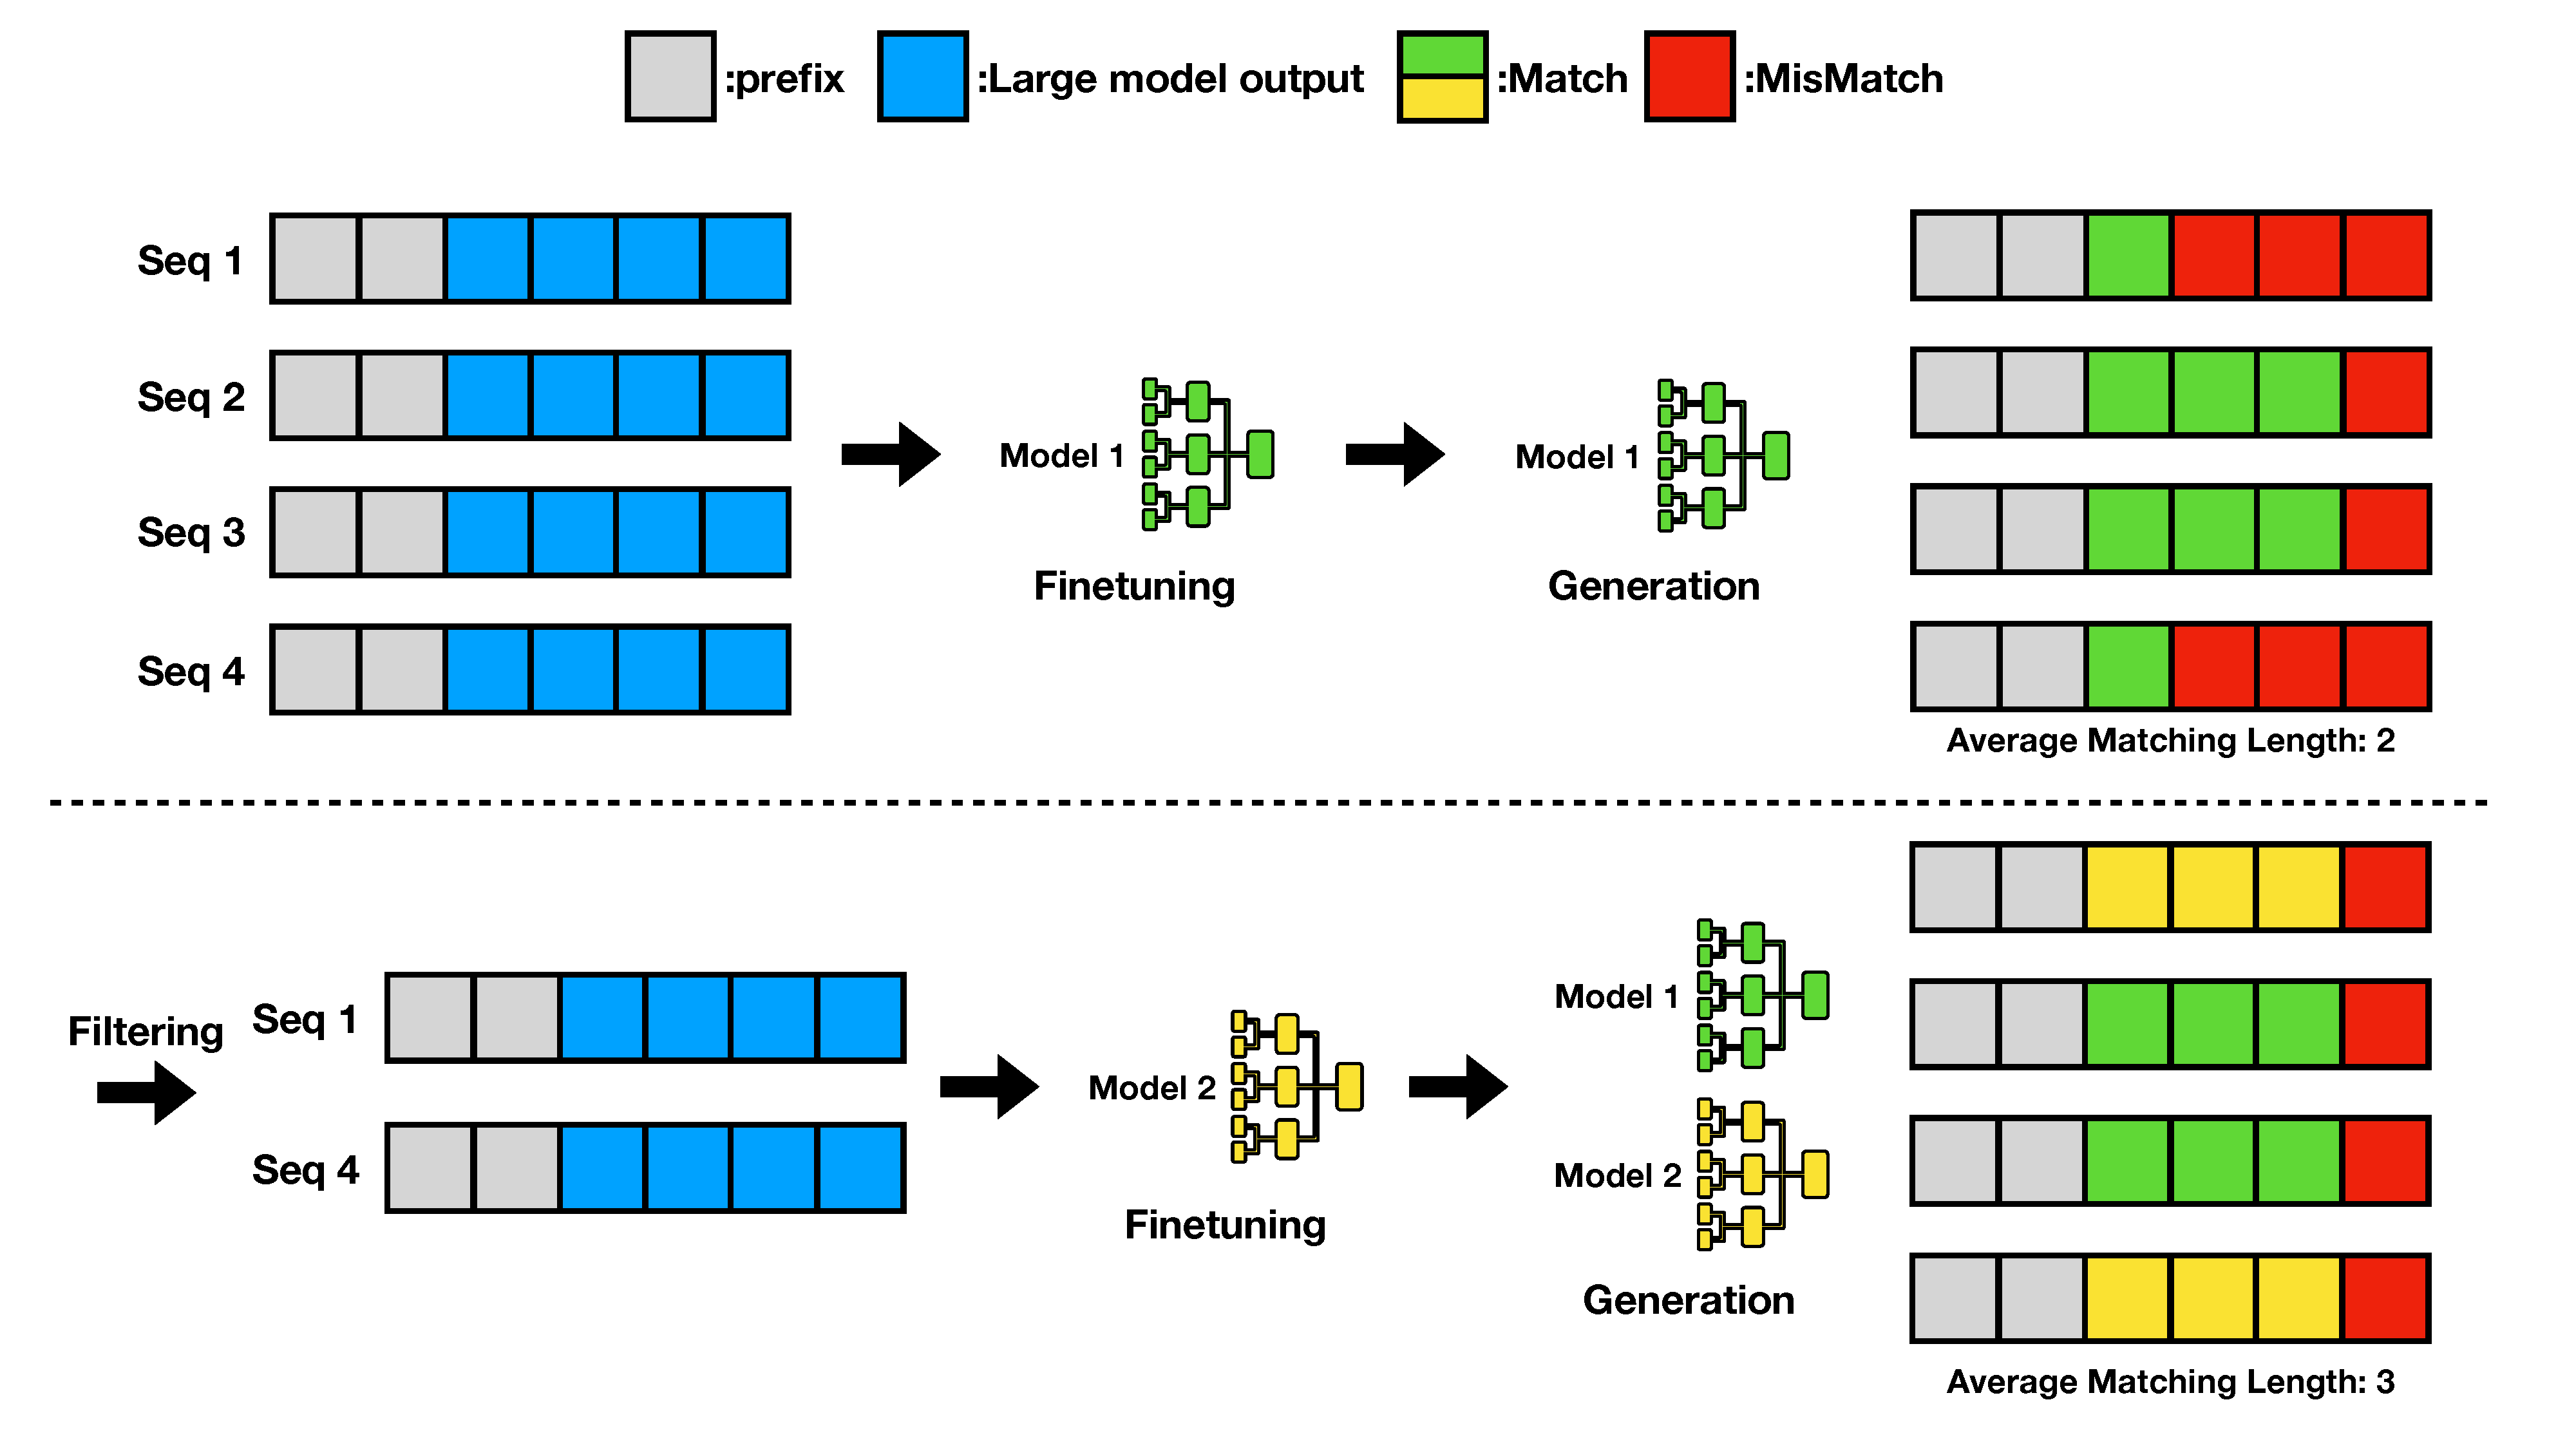
\includegraphics[scale=0.2]{figs/AdaptiveFinetuning.pdf}
    \caption{The process of Collective Boost-Tuning: with only model 1, an average matching length of 2.0 is achieved due to in-accurate alignment between model 1 and the LLM on Seq 1 and 4. However, we can improve the average matching length to 3.0 by adding model 2 which is tuned on Seq 1 and 4.\XM{(Done, to be checked)}}
    \label{fig:CBT}
\end{figure}
\fi 

\if 0
\begin{figure}
    \centering
    %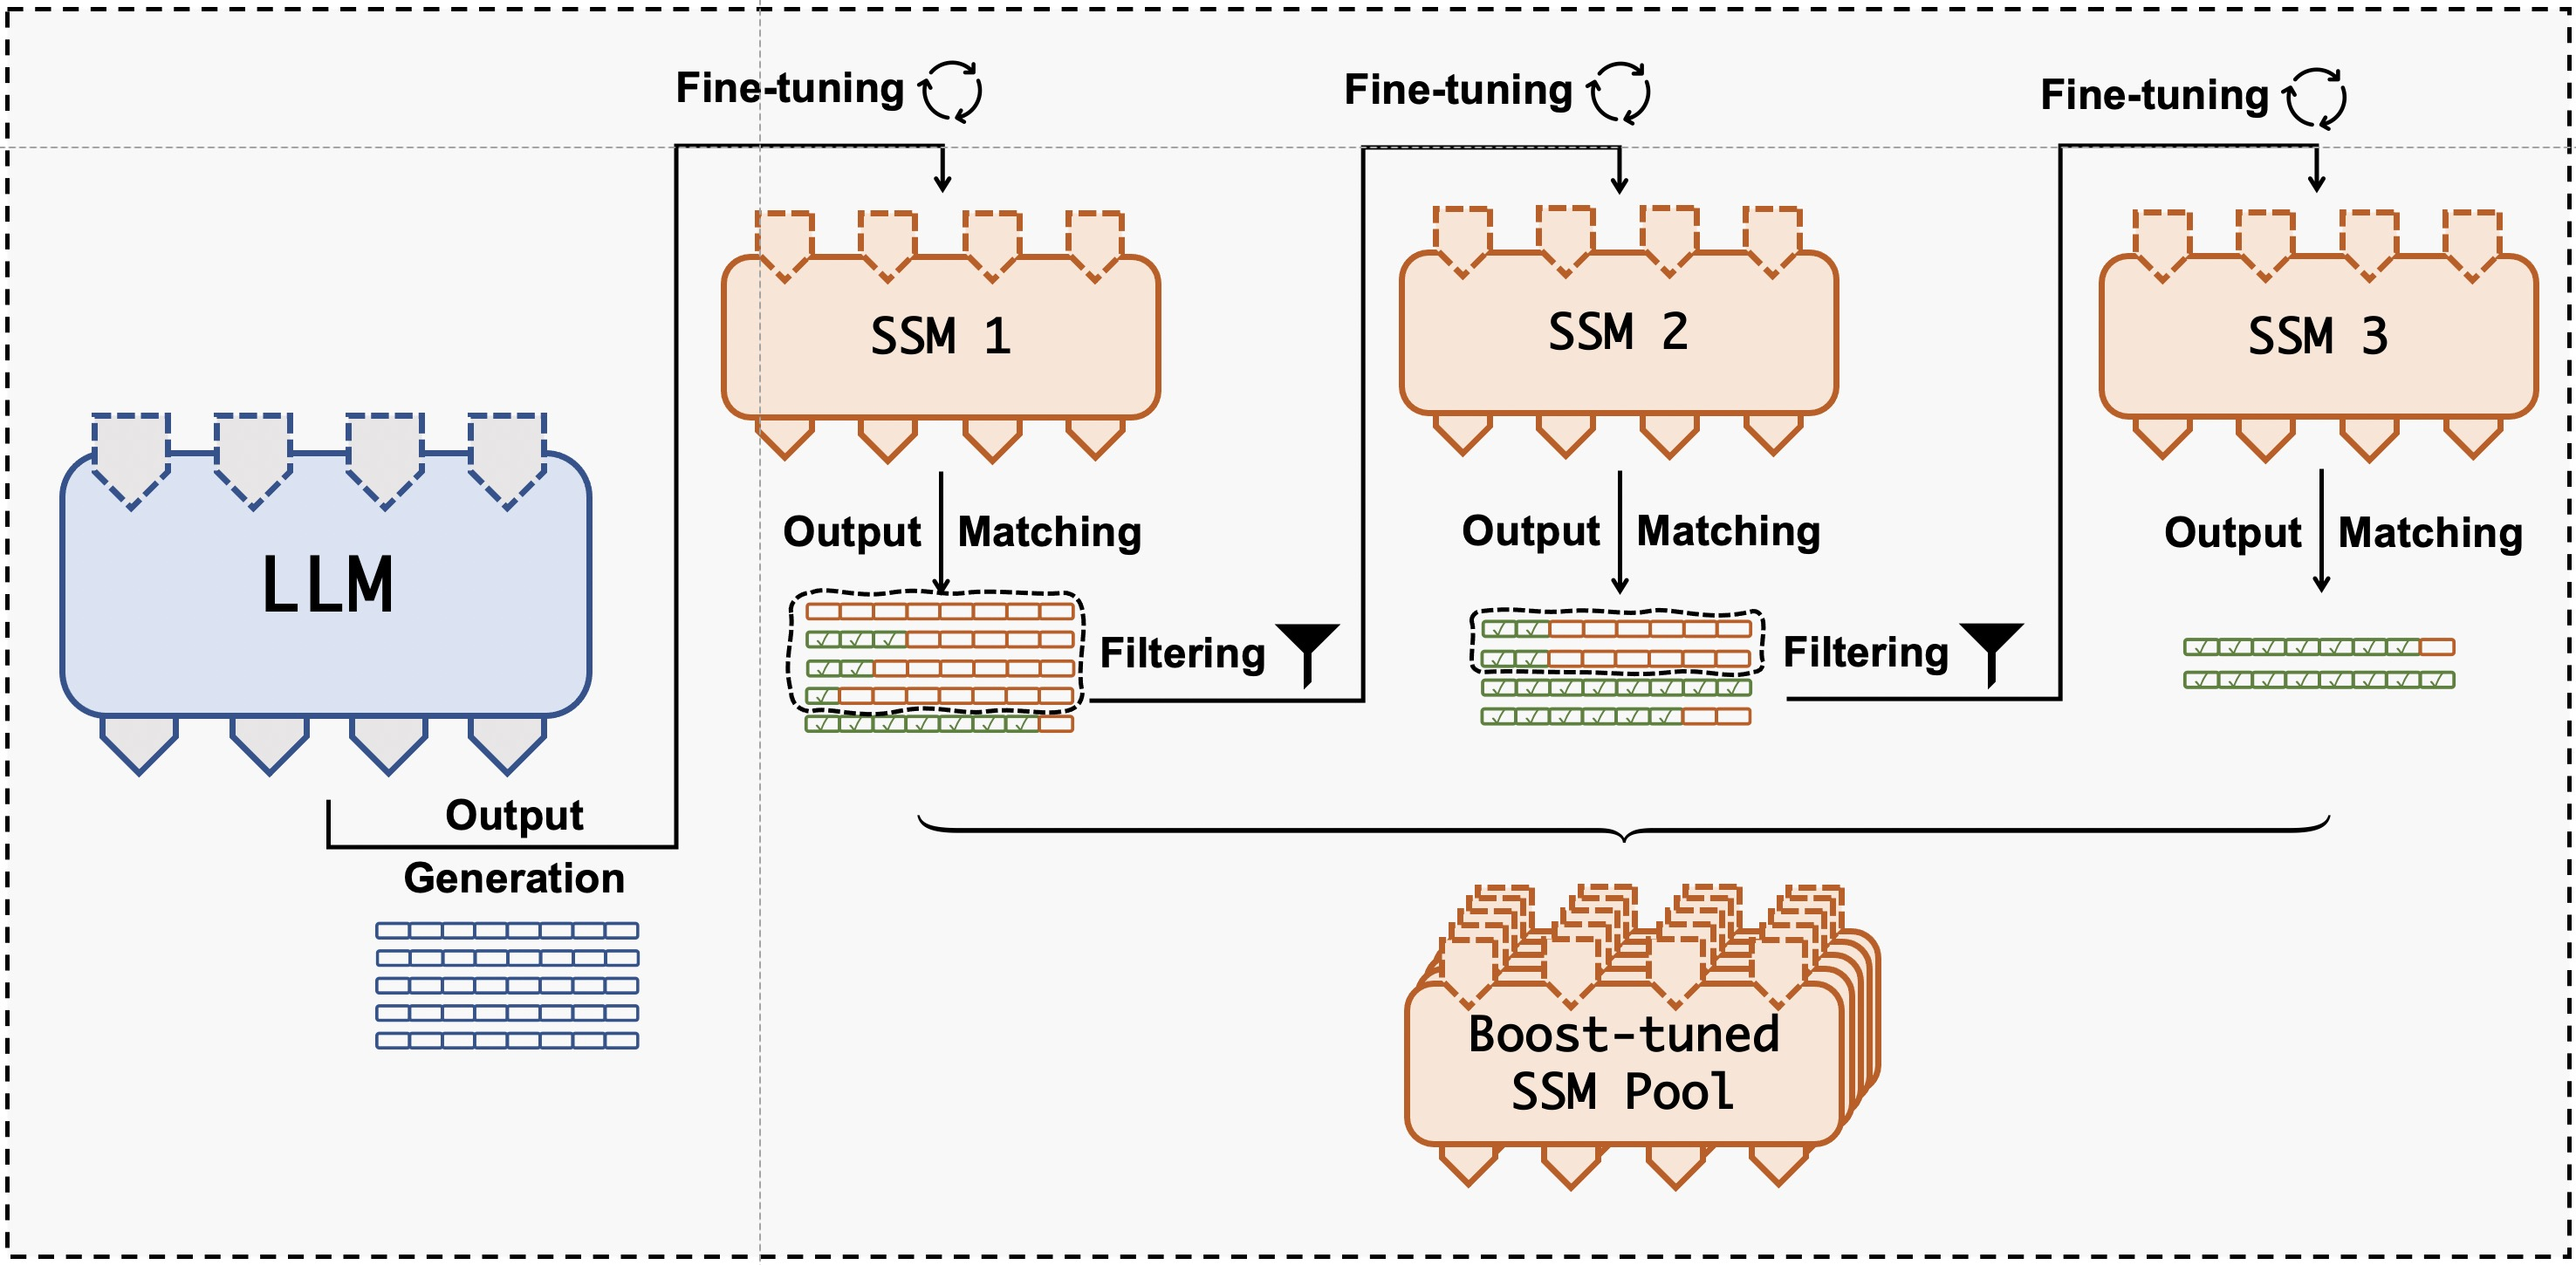
\includegraphics[scale=0.12]{figs/boost_tuning2.jpg}
    %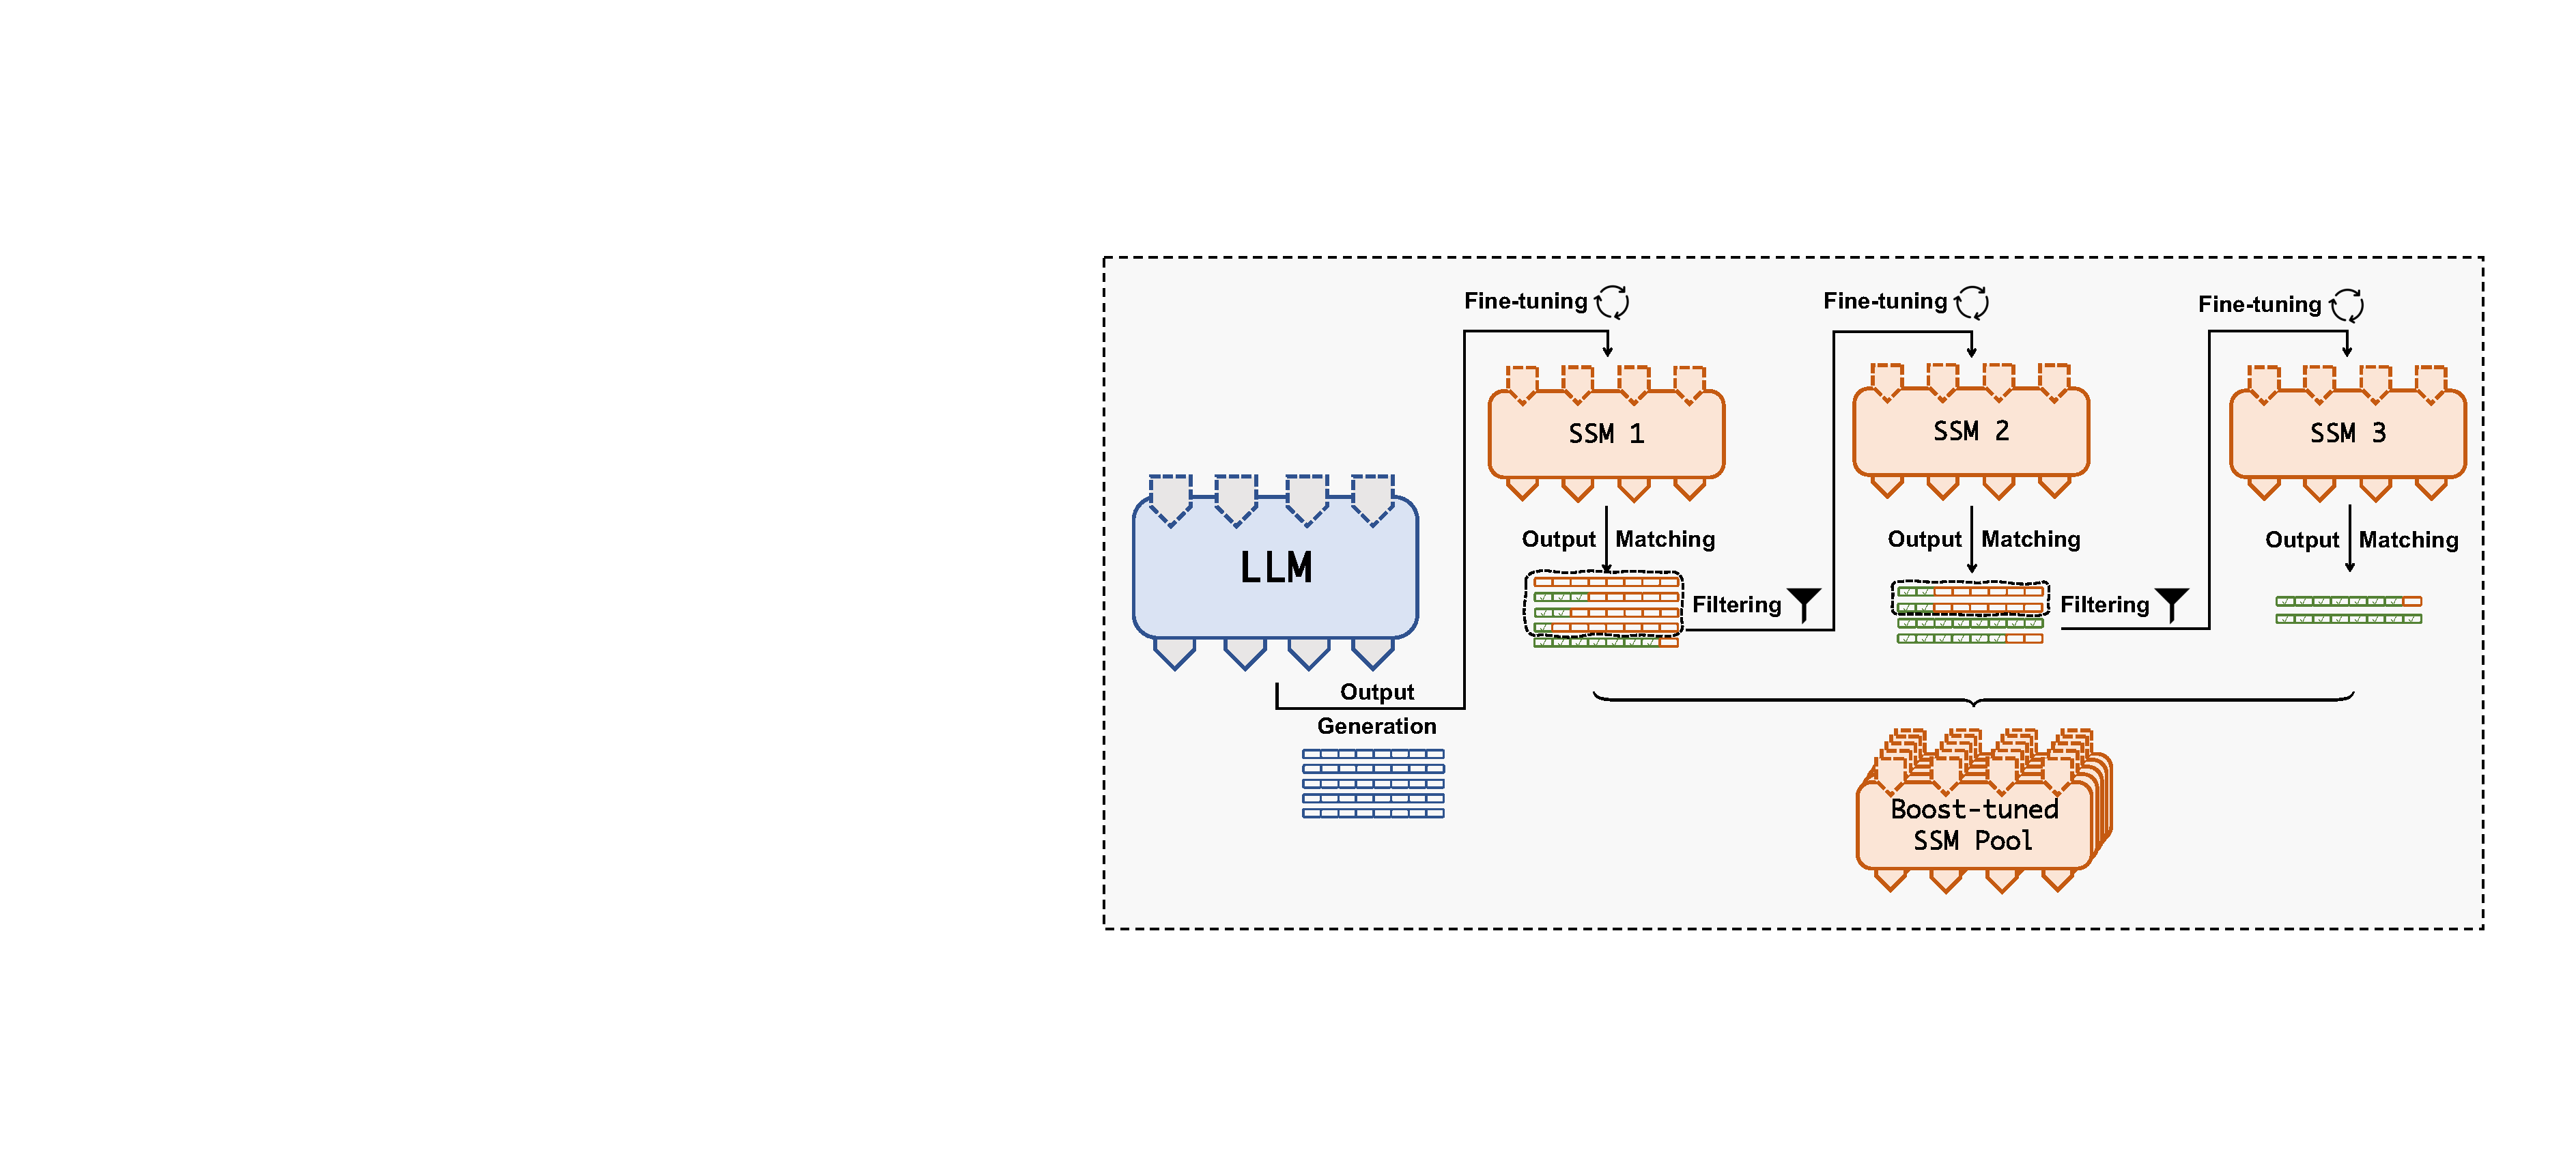
\includegraphics[scale=0.36]{figs/boost_tuning2.pdf}
    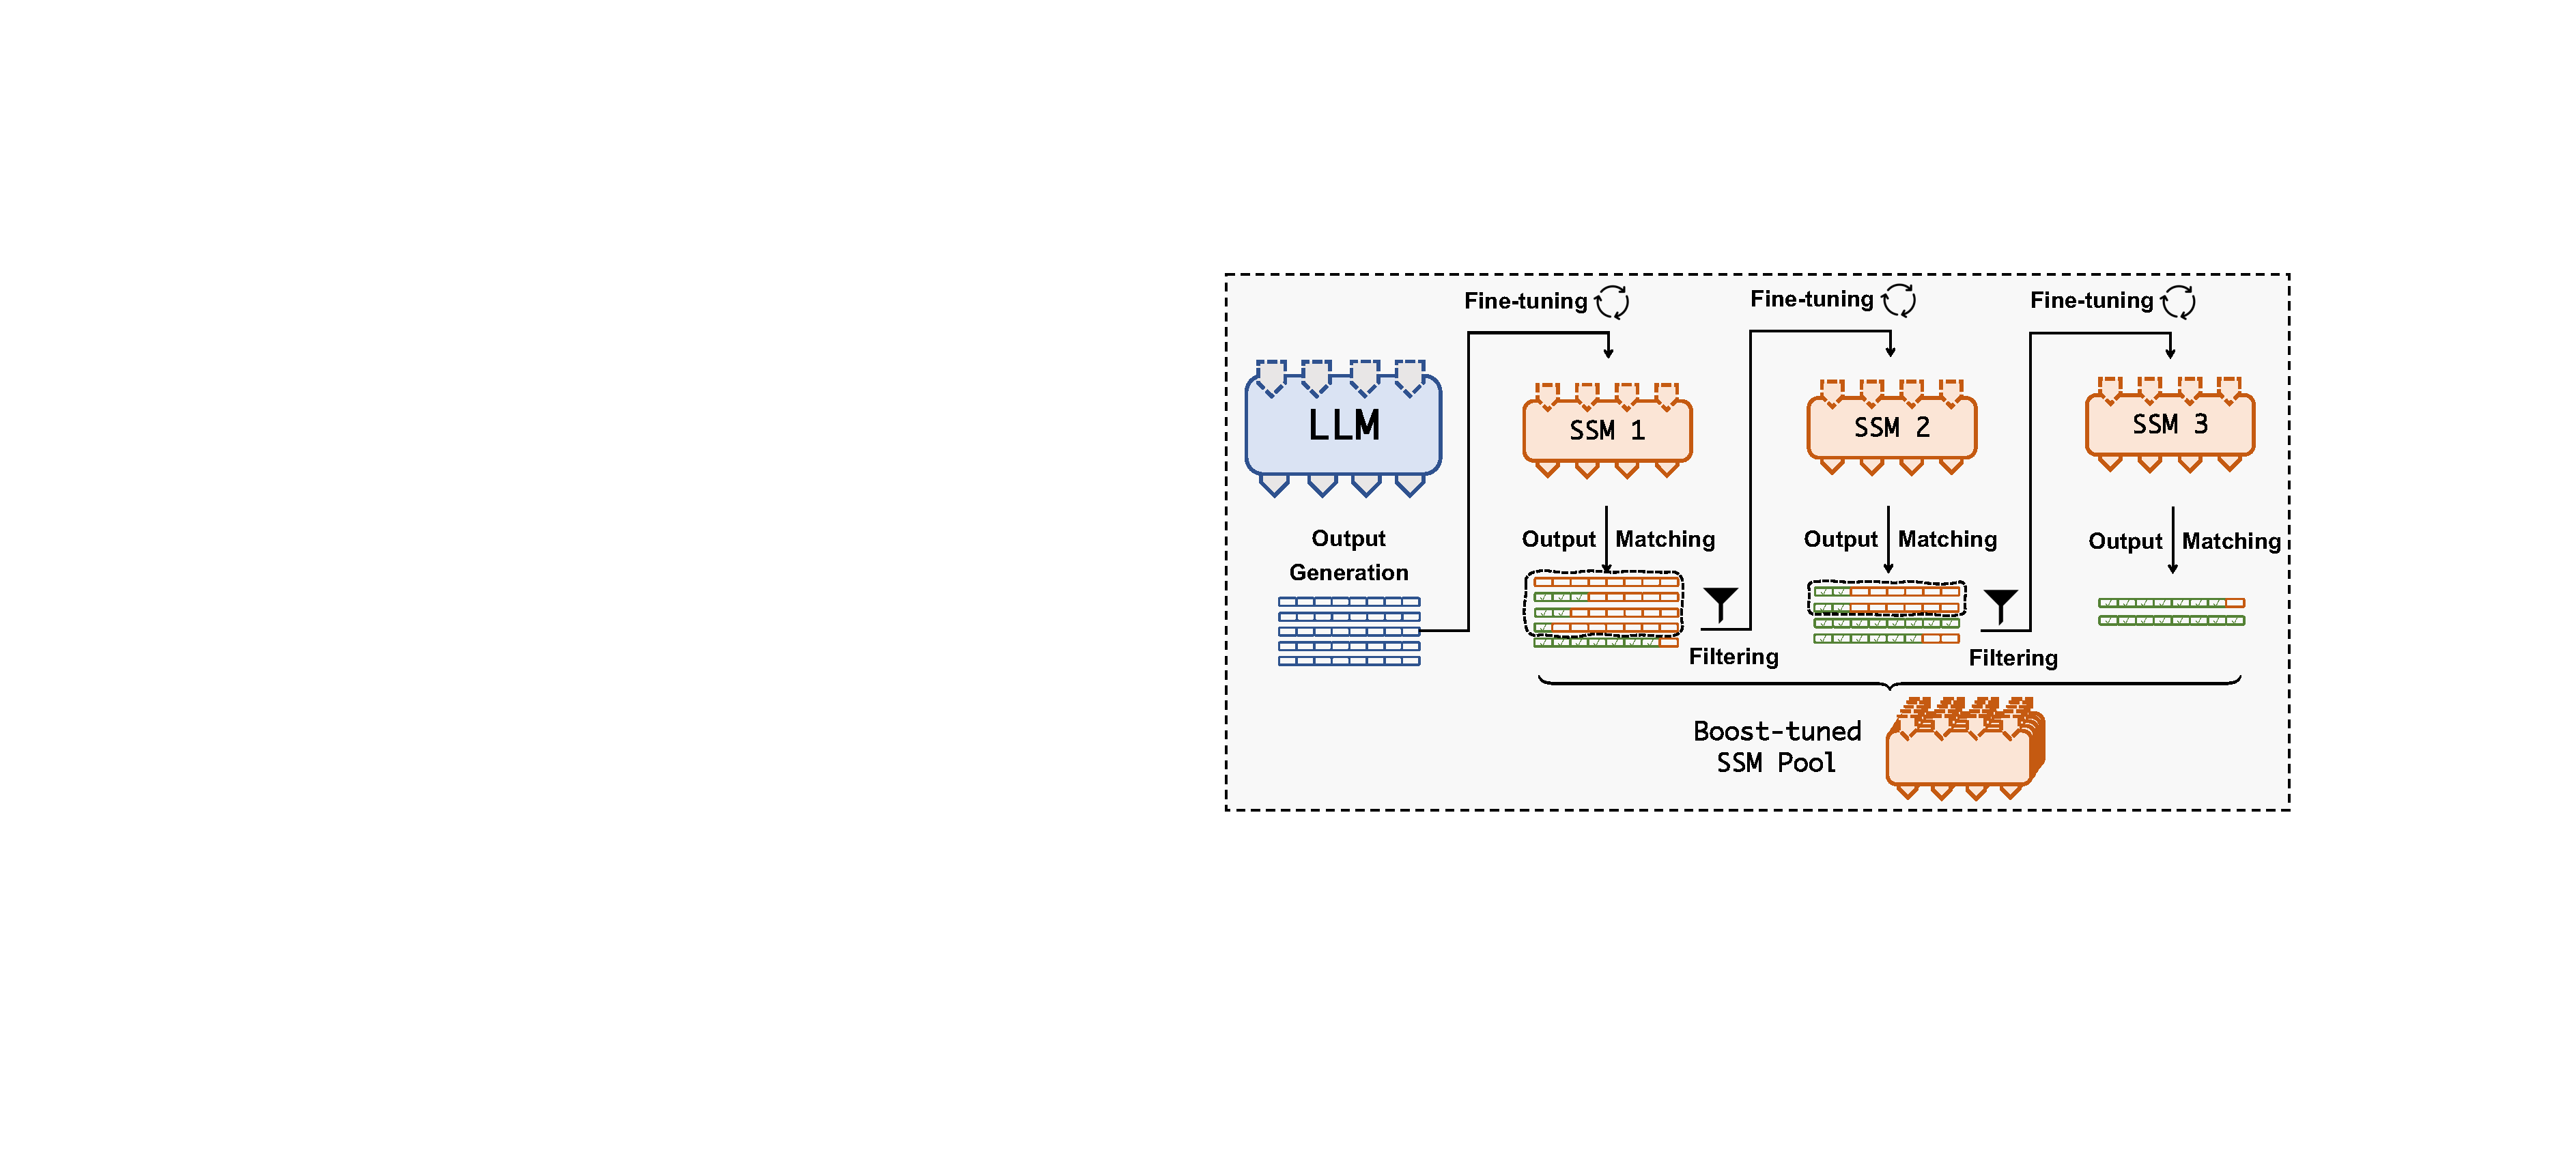
\includegraphics[scale=0.32]{figs/boost_tuning3.pdf}
    \caption{\ZJ{To be removed:} Illustrating \Sys's collective boost-tuning technique. When using a single SSM to generate token trees, \Sys can verify 2.6 tokens on average in each LLM decoding step. This is due to the misalignment between an SSM and LLM on the first four token sequences. By collectively boost-tuning three SSMs, the average number of verified tokens per LLM decoding step is improved to 7.2.}
    \label{fig:CBT}
\end{figure}
\fi

\if 0
\subsection{Learning-based Speculative Scheduler}
\label{sec:LSS}
\ZJ{To be removed.}
To discover an optimal configuration to launch multiple SSMs at each decoding step, we design a {\em learning-based} speculative scheduler that learns to decide which SSMs to use for a given input token sequence and the speculative configurations for these SSMs. 
%%%

%%%
The scheduler includes a matching length predictor and cost model. 
%%%
The matching length predictor takes as input the latest feature representation of the final hidden layer from the LLM and outputs a vector of continuous numbers, each corresponding to the expected matching length under a specific speculative configuration. 
%%%
\Sys uses a three-layer MLP as the neural architecture of the matching length predictor and considers a configuration space of beam search for each SSM, where the beam width $b \in [1, 2, 4]$ and the beam depth $d \in [1, 2, 4, 8, 16]$, therefore the MLP outputs a vector of 15 numbers, each representing the predicted matching length for a speculative configuration.
%%%
The predictor is also trained on publicly available datasets in an offload fashion.
%%%
Note that obtaining the input feature vector for the predictor does not involve extra cost as it's self-contained in the \Sys's verifier (see \Cref{sec:verification}).
%Also, notice that we don't need to pay extra effort to obtain the hidden feature since it's self-contained in the verification engine.
%%%

%%%
To achieve a higher matching length per unit of time, we define the following cost function:
\begin{equation}
    cost(b, d \mid h) = \frac{f(b, d \mid h)}{L_{\text{verify}}(b, d) + L_{\text{speculate}}(b, d) },
    \label{eqn:cost_function}
\end{equation}
where $b$ and $d$ are the beam search width and depth, $h$ is the input feature vector to the predictor, and $f(b, d \mid h)$ is the predicted matching length for the given speculative configuration $(b, d)$ and current context $h$.
%%%
$L_{\text{verify}}(b, d)$ and $L_{\text{speculate}}(b, d)$ are the estimated inference latency for the verifier and speculator, respectively, which are measured by profiling the \Sys runtime system.
%%%
Using the cost function defined in \Cref{eqn:cost_function}, \Sys chooses the configuration that minimizes the expected cost for each SSM:
\begin{equation}
    (b, d) = \arg\max_{(b, d)} cost(b, d \mid h)
\end{equation}
\fi
